% =====================================================================
%  第 4 章 希尔伯特空间上的算子 —— ch04a（§4.1–§4.2）
%  页段：PDF 194–222（原书 p.193–221）
% =====================================================================

\chapter{希尔伯特空间上的算子}

% [原文 p.193]
本章中，$\mathcal{H}$ 表示一个希尔伯特空间。我们始终假定所有希尔伯特空间都是可分的；可分意谓存在可数正交归一基。特别地，任何无穷维的 $\mathcal{H}$ 都酉等价于
\[
\ell^2(\N)=\Bigl\{(a_1,a_2,\cdots,a_n,\cdots)\ \Big|\ a_i\in\C,\ \sum_{i=1}^{\infty}\abs{a_i}^2<\infty\Bigr\}.
\]
我们对两个向量 $\psi,\varphi\in\mathcal{H}$ 的厄米内积采用约定 $\braket{\psi}{\varphi}$，它对第一个变元共轭线性、对第二个变元线性：
\[
\begin{cases}
\braket{\lambda\psi}{\varphi}=\bar\lambda\braket{\psi}{\varphi}\\[1mm]
\braket{\psi}{\lambda\varphi}=\lambda\braket{\psi}{\varphi}
\end{cases}
\qquad \forall\lambda\in\C.
\]
我们写 $\varphi_n\to\varphi$（在 $\mathcal{H}$ 中）表示范数收敛
\[
\lim_{n\to\infty}\norm{\varphi_n-\varphi}=0,
\]
写 $\varphi_n\xrightarrow{\ w\ }\varphi$ 表示弱收敛
\[
\lim_{n\to\infty}\braket{\varphi_n}{\psi}=\braket{\varphi}{\psi},\qquad \forall\psi\in\mathcal{H}.
\]

\section{自伴算子}

\subsection{线性算子}

\begin{definition}{4.1.1}
  $\mathcal{H}$ 上的线性算子 $A$ 是指线性映射
  \[
  A:\Dom(A)\longrightarrow\mathcal{H},
  \]
  其中 $\Dom(A)\subset\mathcal{H}$ 称为 $A$ 的定义域。$A$ 的像称为它的值域，记作 $\Ran(A)$。对 $\mathcal{H}$ 上的两个线性算子，若 $\Dom(A)\subset\Dom(B)$ 且
  \[
  A\varphi=B\varphi,\qquad\forall\varphi\in\Dom(A),
  \]
  则记 $A\subseteq B$。算子 $B$ 称为 $A$ 的扩张。若 $A\subseteq B$ 且 $B\subseteq A$，则记 $A=B$。
\end{definition}

除另有说明外，本讲义中“算子”一词总是指线性算子。

% [原文 p.194]
\begin{definition}{4.1.2}
  算子 $A$ 的算子范数定义为
  \[
  \norm{A}=\sup_{\norm{\varphi}=1}\norm{A\varphi}.
  \]
  若 $\norm{A}<+\infty$，则称 $A$ 是有界的。对有界算子，我们总可以假定 $\Dom(A)=\mathcal{H}$。$\mathcal{H}$ 上全体有界线性算子连同算子范数构成一个巴拿赫空间，我们记作 $\mathbf{B}(\mathcal{H})$。
\end{definition}

我们在量子力学中会经常遇到无界算子。例如哈密顿算子往往是无界的。给定两个算子 $A_1$ 与 $A_2$，我们定义
\begin{itemize}[leftmargin=2em,itemsep=1pt]
  \item $(A_1+A_2)(\varphi)=A_1\varphi+A_2\varphi$，对 $\varphi\in\Dom(A_1)\cap\Dom(A_2)$；
  \item $A_1A_2(\varphi)=A_1(A_2(\varphi))$，对 $\varphi\in A_2^{-1}(\Dom(A_1))$。
\end{itemize}

\begin{example}{4.1.3}
  设 $\mathcal{H}=L^2(\R^n)$。给定 $\R^n$ 上的可测函数 $f(\mathbf{x})$，用乘以 $f$ 的方式定义 $L^2(\R^n)$ 上的线性算子 $M_f$
  \[
  M_f:\varphi\longmapsto f\varphi.
  \]
  $M_f$ 的定义域是
  \[
  \Dom(M_f)=\{\varphi\in L^2(\R^n)\mid f\varphi\in L^2(\R^n)\}.
  \]
  断言：$M_f$ 有界 $\iff\norm{f}_{L^\infty}<\infty$。$M_f$ 的算子范数是
  \[
  \norm{M_f}=\norm{f}_{L^\infty}.
  \]

  \begin{proof}
    （$\Leftarrow$）设 $\norm{f}_{L^\infty}=C<\infty$。则对一切 $\varphi\in L^2(\R^n)$，
    \[
    \int_{\R^n}\abs{f\varphi}^2\rd\mathbf{x}\le C^2\int_{\R^n}\abs{\varphi}^2\rd\mathbf{x},
    \]
    故 $\norm{M_f\varphi}_{L^2}\le C\norm{\varphi}_{L^2}$。这说明 $M_f$ 有界，且 $\norm{M_f}\le\norm{f}_{L^\infty}$。

    （$\Rightarrow$）设 $M_f$ 有界，$\norm{M_f}=C$。令
    \[
    \chi_k(\mathbf{x})=\begin{cases}1&\text{若 } \abs{f(\mathbf{x})}\le k,\\[1mm] 0&\text{若 } \abs{f(\mathbf{x})}>k,\end{cases}
    \]
    并考虑 $\varphi_k(\mathbf{x})=(1-\chi_k(\mathbf{x}))\ee^{-\abs{\mathbf{x}}^2}$。则 $\varphi_k\in L^2(\R^n)$，且
    \[
    k\norm{\varphi_k}_{L^2}\le\norm{M_f\varphi_k}_{L^2}\le\norm{M_f}\norm{\varphi_k}_{L^2}.
    \]
    于是当 $k>\norm{M_f}$ 时 $\varphi_k=0$ 几乎处处，从而 $\norm{f}_{L^\infty}\le\norm{M_f}$。
  \end{proof}

  当 $\norm{f}_{L^\infty}=\infty$ 时，对任意 $\varphi\in L^2(\R^n)$，考虑
  \[
  \varphi_k(\mathbf{x})=\varphi(\mathbf{x})\chi_k(\mathbf{x}),
  \]
  其中 $\chi_k(\mathbf{x})$ 如上定义。则 $\varphi_k\in\Dom(M_f)$，且由控制收敛定理
  \[
  \lim_{k\to\infty}\varphi_k=\varphi\qquad\text{在 } L^2(\R^n)\text{ 中}.
  \]
  这说明定义域 $\Dom(M_f)$ 在 $L^2(\R^n)$ 中稠密。
\end{example}

% [原文 p.195]
\subsection{图像与闭性}

\begin{definition}{4.1.4}
  $\mathcal{H}$ 上算子 $A$ 的图像 $\Gamma(A)$ 是
  \[
  \Gamma(A)=\{(\varphi,A\varphi)\mid\varphi\in\Dom(A)\}\subset\mathcal{H}^2.
  \]
  若 $\Gamma(A)$ 是 $\mathcal{H}^2$ 的闭子集，则称 $A$ 是闭的。若闭包 $\overline{\Gamma(A)}$ 是某个算子 $\overline{A}$ 的图像：
  \[
  \Gamma(\overline{A})=\overline{\Gamma(A)},
  \]
  则称 $A$ 是可闭的。此时 $\overline{A}$ 称为 $A$ 的闭包。具体地说，若序列 $(\varphi_n,A\varphi_n)\to(\varphi,\tilde\varphi)$ 在 $\mathcal{H}^2$ 中，则 $\tilde\varphi$ 应由 $\varphi$ 唯一确定，而 $\overline{A}$ 由 $\overline{A}\varphi=\tilde\varphi$ 定义。
\end{definition}

等价地，若存在 $\Dom(A)$ 中的序列 $\varphi_n$ 使得
\[
\varphi_n\to 0,\qquad\text{但 } A\varphi_n\to\tilde\varphi\ne 0,
\]
则 $A$ 不可闭。

\begin{theorem}{4.1.5}
  （闭图像定理）定义在整个 $\mathcal{H}$ 上的算子 $A$ 是闭的，当且仅当 $A$ 有界。
\end{theorem}

\begin{example}{4.1.6}
  设 $\mathcal{H}=L^2([0,1])$，考虑算子
  \[
  A\varphi=\varphi(0),\qquad\Dom(A)=C([0,1]),
  \]
  于是 $A$ 的值域是常数函数。考虑
  \[
  \varphi_n=\begin{cases}1-nx&0\le x\le\dfrac1n,\\[2mm] 0&\dfrac1n\le x\le 1.\end{cases}
  \]

  \begin{center}
    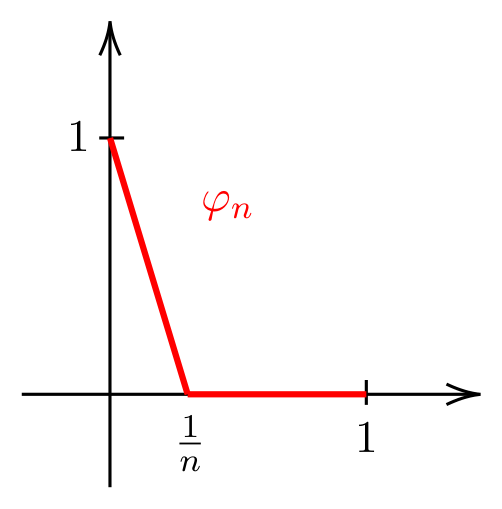
\includegraphics[width=0.34\textwidth]{figures/fig_p196_a.png}
  \end{center}
  % [图：原书 p.195，图内文字照原样保留]

  则 $\varphi_n\to 0$ 在 $L^2([0,1])$ 中，但 $A\varphi_n\to 1$。故 $A$ 是不可闭算子。
\end{example}

\subsection{伴随算子}

\begin{definition}{4.1.7}
  设 $A$ 是希尔伯特空间 $\mathcal{H}$ 上定义域 $\Dom(A)$ 稠密的线性算子。$A$ 的伴随 $A^*$ 定义为
  \[
  A^*:\Dom(A^*)\longrightarrow\mathcal{H},
  \]
  其中
  \[
  \Dom(A^*)=\{\varphi\in\mathcal{H}\mid\exists\tilde\varphi\in\mathcal{H}:\ \braket{\varphi}{A\psi}=\braket{\tilde\varphi}{\psi},\ \forall\psi\in\Dom(A)\},
  \]
  而对如上所述的 $\tilde\varphi$，$A^*\varphi=\tilde\varphi$。$\Dom(A)$ 的稠密性蕴含：当 $\varphi\in\Dom(A^*)$ 时，这样的 $\tilde\varphi$ 唯一确定。
\end{definition}

% [原文 p.196]
伴随 $A^*$ 也可用算子的图像来等价描述。我们把 $\mathcal{H}^2$ 中的内积记作
\[
\ip{(u_1,v_1)}{(u_2,v_2)}=\braket{u_1}{u_2}+\braket{v_1}{v_2},\qquad u_i,v_i\in\mathcal{H}.
\]
定义关系 $A^*\varphi=\tilde\varphi$ 可表述为
\[
\ip{(\varphi,\tilde\varphi)}{(-A\psi,\psi)}=0,\qquad\forall\psi\in\Dom(A).
\]
在 $\mathcal{H}^2$ 上引入酉算子 $J$
\[
J(u,v)=(-v,u).
\]
则上述关系可以写成
\[
\Gamma(A^*)=(J\Gamma(A))^\perp.
\]

\begin{proposition}{4.1.8}
  设 $A$ 是 $\mathcal{H}$ 上稠密定义的算子。则
  \begin{enumerate}[label=\textcircled{\small\arabic*},leftmargin=2.6em,itemsep=2pt]
    \item $A^*$ 是闭的。
    \item $A$ 可闭，当且仅当 $\Dom(A^*)$ 稠密。此时 $\overline{A}=A^{**}$，即双重伴随。
    \item $\Ker A^*=\Ran(A)^\perp$。
  \end{enumerate}
\end{proposition}

\begin{proof}
  \textcircled{\small 1} $\Gamma(A^*)=(J\Gamma(A))^\perp$ 说明 $\Gamma(A^*)$ 是闭的。

  \textcircled{\small 2} 关系 $\Gamma(A^*)=(J\Gamma(A))^\perp$ 蕴含 $\overline{\Gamma(A)}=(J\Gamma(A^*))^\perp$。设 $(0,\xi)\in\overline{\Gamma(A)}$，则
  \[
  \braket{\varphi}{\xi}=\braket{A^*\varphi}{0},\qquad\forall\varphi\in\Dom(A^*),
  \]
  即 $\xi\in\Dom(A^*)^\perp$。于是 $A$ 可闭，当且仅当 $\Dom(A^*)$ 稠密；由此推出 $\xi=0$。此时 $\overline{\Gamma(A)}=(J\Gamma(A^*))^\perp=\Gamma(A^{**})$，故 $\overline{A}=A^{**}$。

  \textcircled{\small 3} 若
  \[
  \braket{\varphi}{A\psi}=\braket{0}{\psi}=0,\qquad\forall\psi\in\Dom(A),
  \]
  则 $A^*\varphi=0$，即 $\varphi\in\Ran(A)^\perp$。
\end{proof}

\begin{example}{4.1.9}
  考虑 $L^2(\R^n)$ 上乘以可测函数 $f(\mathbf{x})$ 的算子 $M_f$。则
  \[
  M_f^*=M_{\bar f}.
  \]
  事实上，对任意 $\varphi_1,\varphi_2\in\Dom(M_f)$，
  \[
  \braket{\varphi_1}{M_f\varphi_2}
  =\int_{\R^n}\overline{\varphi_1(\mathbf{x})}f(\mathbf{x})\varphi_2(\mathbf{x})\rd\mathbf{x}
  =\int_{\R^n}\overline{\bar f\varphi_1(\mathbf{x})}\varphi_2(\mathbf{x})\rd\mathbf{x}
  =\mel{M_{\bar f}\varphi_1}{}{\varphi_2}.
  \]
  这说明
  \[
  M_f^*\varphi=M_{\bar f}\varphi,\qquad\forall\varphi\in\Dom(M_f)
  \quad\Longrightarrow\quad
  M_{\bar f}\subseteq M_f^*.
  \]
  \tutornote{原文此处写 $\forall\varphi\in\Dom(A)$，但例中只出现 $M_f$，$A$ 未定义；按上下文应为 $\Dom(M_f)$。}

  % [原文 p.197]
  另一方面，设 $\varphi_1\in\Dom(M_f^*)$，即存在 $\tilde\varphi_1\in L^2(\R^n)$ 使得
  \[
  \int_{\R^n}\overline{\varphi_1(\mathbf{x})}f(\mathbf{x})\varphi_2(\mathbf{x})\rd\mathbf{x}
  =\int_{\R^n}\overline{\tilde\varphi_1(\mathbf{x})}\varphi_2(\mathbf{x})\rd\mathbf{x},
  \qquad\forall\varphi_2\in\Dom(M_f).
  \]
  令
  \[
  \chi_k(\mathbf{x})=\begin{cases}1&\text{若 } \abs{f(\mathbf{x})}\le k,\\[1mm] 0&\text{若 } \abs{f(\mathbf{x})}>k.\end{cases}
  \]
  则对任意 $g\in L^2(\R^n)$，$\chi_kg\in\Dom(M_f)$。因此
  \[
  \int_{\R^n}\Bigl(\overline{\varphi_1}f-\overline{\tilde\varphi_1}\Bigr)\chi_kg\,\rd\mathbf{x}=0,
  \qquad\forall g\in L^2(\R^n)
  \]
  \[
  \Longrightarrow\quad
  \Bigl(\overline{\varphi_1}f-\overline{\tilde\varphi_1}\Bigr)\chi_k=0
  \qquad\text{在 } L^2(\R^n)\text{ 中}.
  \]
  这对任意 $k$ 成立，故推出
  \[
  f\overline{\varphi_1}=\overline{\tilde\varphi_1}\quad\text{在 } L^2(\R^n)\text{ 中}
  \quad\Longrightarrow\quad
  \varphi_1\in\Dom(M_{\bar f}).
  \]
  这说明 $M_f^*\subseteq M_{\bar f}$。
\end{example}

\subsection{对称算子与自伴算子}

\begin{definition}{4.1.10}
  稠密定义的线性算子 $A$ 称为自伴的，若 $A=A^*$。
\end{definition}

由例 4.1.9，若 $f$ 是实可测函数，则 $M_f$ 是自伴的。

\begin{definition}{4.1.11}
  稠密定义的线性算子 $A$ 称为对称的，若
  \[
  \braket{\varphi_1}{A\varphi_2}=\braket{A\varphi_1}{\varphi_2},\qquad\varphi_1,\varphi_2\in\Dom(A).
  \]
\end{definition}

显然，对称算子 $A$ 满足
\[
A\subseteq A^*.
\]
因此对称算子是比自伴算子更弱的概念。

\begin{proposition}{4.1.12}
  算子 $A$ 是对称算子，当且仅当
  \[
  \braket{\varphi}{A\varphi}\in\R,\qquad\forall\varphi\in\Dom(A).
  \]
\end{proposition}

\begin{proof}
  若 $A$ 是对称算子，则
  \[
  \overline{\braket{\varphi}{A\varphi}}=\braket{A\varphi}{\varphi}=\braket{\varphi}{A\varphi}
  \quad\Longrightarrow\quad
  \braket{\varphi}{A\varphi}\in\R.
  \]
  反之，对任意 $\varphi_1,\varphi_2\in\Dom(A)$，比较等式
  \[
  \braket{\varphi_1+\ii\varphi_2}{A(\varphi_1+\ii\varphi_2)}
  =\braket{\varphi_1}{A\varphi_1}+\braket{\varphi_2}{A\varphi_2}
  +\ii\braket{\varphi_1}{A\varphi_2}-\ii\braket{\varphi_2}{A\varphi_1}
  \]
  的虚部，我们得到
  \[
  \Real\bigl(\braket{\varphi_1}{A\varphi_2}\bigr)
  =\Real\bigl(\braket{\varphi_2}{A\varphi_1}\bigr)
  =\Real\bigl(\braket{A\varphi_1}{\varphi_2}\bigr).
  \]
  把 $\varphi_2$ 换成 $\ii\varphi_2$，该恒等式给出
  \[
  \Imag\bigl(\braket{\varphi_1}{A\varphi_2}\bigr)=\Imag\bigl(\braket{A\varphi_1}{\varphi_2}\bigr).
  \]
  于是 $\braket{\varphi_1}{A\varphi_2}=\braket{A\varphi_1}{\varphi_2}$，$A$ 是对称算子。
\end{proof}

% [原文 p.198]
\begin{example}{4.1.13}
  设希尔伯特空间 $\mathcal{H}=L^2([0,1])$。定义算子（$\hbar=1$ 时的动量算子）
  \[
  A\varphi=-\ii\frac{\rd}{\rd x}\varphi,
  \]
  其定义域为
  \[
  \Dom(A)=\{\varphi\in C^1([0,1])\mid\varphi(0)=\varphi(1)=0\}.
  \]
  对任意 $\varphi_1,\varphi_2\in\Dom(A)$，用分部积分，
  \[
  \braket{\varphi_1}{A\varphi_2}
  =\int_0^1\overline{\varphi_1}\Bigl(-\ii\frac{\rd}{\rd x}\Bigr)\varphi_2\rd x
  =\int_0^1\overline{-\ii\frac{\rd}{\rd x}\varphi_1}\,\varphi_2\rd x
  -\ii\overline{\varphi_1}\varphi_2\Big|_0^1
  =\braket{A\varphi_1}{\varphi_2}.
  \]
  因此 $A$ 是对称算子。

  下面计算 $A^*$。设 $\varphi\in\Dom(A^*)$，即存在 $\tilde\varphi\in L^2([0,1])$ 使得
  \[
  \int_0^1\bar\varphi\,(-\ii f')\rd x=\int_0^1\overline{\tilde\varphi}\,f\rd x,
  \qquad\forall f\in\Dom(A).
  \]
  由于 $\tilde\varphi$ 在 $[0,1]$ 上可积、$f$ 绝对连续，分部积分给出
  \[
  \int_0^1\bar\varphi f\rd x=-\int_0^1\Bigl(\int_0^x\bar\varphi\Bigr)f'\rd x.
  \]
  于是
  \[
  \int_0^1\Bigl(\varphi(x)-\ii\int_0^x\tilde\varphi\Bigr)f'(x)\rd x=0,
  \qquad\forall f\in\Dom(A)
  \]
  \[
  \Longrightarrow\quad
  \varphi(x)-\ii\int_0^x\tilde\varphi\ \in\ \{f'\mid f\in\Dom(A)\}^{\perp}.
  \]
  另一方面，
  \[
  \{f'\mid f\in\Dom(A)\}=\Bigl\{g\in C([0,1])\ \Big|\ \int_0^1 g\,\rd x=0\Bigr\}
  =\{g\in C([0,1])\mid\braket{1}{g}=0\}
  \]
  \[
  \Longrightarrow\quad
  \overline{\{f'\mid f\in\Dom(A)\}}=\{g\in L^2([0,1])\mid\braket{1}{g}=0\}=\{1\}^{\perp}
  \]
  \[
  \Longrightarrow\quad
  \{f'\mid f\in\Dom(A)\}^{\perp}=\C.
  \]
  由此可知 $\varphi(x)-\ii\int_0^x\tilde\varphi$ 是常数函数，于是
  \[
  \varphi(x)=\varphi(0)+\ii\int_0^x\tilde\varphi.
  \]
  因此
  \[
  \varphi\in H^1([0,1])=\bigl\{f(x)\ \big|\ \text{在 }[0,1]\text{ 上绝对连续，且 } f'(x)\in L^2([0,1])\bigr\}.
  \]
  反之，给定任意 $\varphi\in H^1([0,1])$，
  \[
  \varphi(x)=\varphi(0)+\ii\int_0^x\varphi'\rd x,\qquad\varphi'\in L^2([0,1]).
  \]
  把上述论证倒过来，我们得到 $A^*\varphi=-\ii\varphi'$。因此
  \[
  \Dom(A^*)=H^1([0,1]).
  \]
  此时 $A\subsetneq A^*$，即 $A$ 是对称算子，但不是自伴算子。
\end{example}

% [原文 p.199]
\begin{proposition}{4.1.14}
  $A\subseteq B\ \Longrightarrow\ B^*\subseteq A^*$。
\end{proposition}

\begin{proof}
  显然。
\end{proof}

\begin{corollary}{4.1.15}
  设 $A$ 自伴、$B$ 对称，且 $A\subseteq B$。则 $A=B$。换言之，自伴算子关于对称扩张是极大的。
\end{corollary}

\begin{proof}
  由于 $B$ 对称，$B\subseteq B^*$。于是
  \[
  A\subseteq B\subseteq B^*\subseteq A^*=A
  \quad\Longrightarrow\quad
  A=B.
  \]
\end{proof}

\begin{proposition}{4.1.16}
  设 $A$ 是 $\mathcal{H}$ 上稠密定义的对称算子。则 $A$ 可闭。
\end{proposition}

\begin{proof}
  若 $A$ 对称，则 $A\subseteq A^*$，故 $A^*$ 稠密定义。由命题 4.1.8，$A$ 可闭，且 $\overline{A}=A^{**}$。注意
  \[
  A\subseteq A^{**}\subseteq A^*,
  \]
  而闭包 $\overline{A}=A^{**}$ 是 $A$ 的对称扩张。
\end{proof}

\begin{example}{4.1.17}
  （例 4.1.13 续）$\mathcal{H}=L^2([0,1])$，且
  \[
  A=-\ii\frac{\rd}{\rd x},\qquad
  \Dom(A)=\{\varphi\in C^1([0,1])\mid\varphi(0)=\varphi(1)=0\}.
  \]
  考虑算子
  \[
  B=-\ii\frac{\rd}{\rd x},\qquad
  \Dom(B)=\{\varphi\in C^1([0,1])\mid\varphi(0)=\varphi(1)\}.
  \]
  显然 $A\subseteq B$。对任意 $\varphi_1,\varphi_2\in\Dom(B)$，
  \[
  \begin{aligned}
  \braket{\varphi_1}{B\varphi_2}
  &=\int_0^1\overline{\varphi_1(x)}\Bigl(-\ii\frac{\rd}{\rd x}\varphi_2\Bigr)\rd x\\
  &=\int_0^1\overline{\Bigl(-\ii\frac{\rd}{\rd x}\varphi_1\Bigr)}\varphi_2\rd x
  -\ii\varphi_1\overline{\varphi_2}\Big|_0^1\\
  &=\int_0^1\overline{\Bigl(-\ii\frac{\rd}{\rd x}\varphi_1\Bigr)}\varphi_2\rd x\\
  &=\braket{B\varphi_1}{\varphi_2}.
  \end{aligned}
  \]
  故 $B$ 是 $A$ 的对称扩张。

  下面计算 $B^*$。由于 $B^*\subseteq A^*$，
  \[
  \Dom(B^*)\subseteq\Dom(A^*)=H^1([0,1]).
  \]
  设 $\varphi\in\Dom(B^*)$，则
  \[
  \int_0^1\bar\varphi f'\rd x=\int_0^1\overline{\varphi'}f\rd x,\qquad\forall f\in\Dom(B)
  \]

  % [原文 p.200]
  用分部积分
  \[
  \Longrightarrow\quad \bar\varphi f\Big|_0^1=0,\quad\forall f\in\Dom(B)
  \qquad\Longrightarrow\quad \varphi(0)=\varphi(1).
  \]
  因此
  \[
  \Dom(B^*)=\{\varphi\in H^1([0,1])\mid\varphi(0)=\varphi(1)\}.
  \]
  类似的计算给出
  \[
  \Dom(B^{**})=\{\varphi\in H^1([0,1])\mid\varphi(0)=\varphi(1)\}.
  \]
  故 $B^*=\overline{B}$ 是自伴算子。于是 $\overline{B}$ 是 $A$ 的极大对称扩张。
\end{example}

\begin{proposition}{4.1.18}
  若对称算子 $A$ 定义在整个 $\mathcal{H}$ 上，则 $A$ 有界。
\end{proposition}

\begin{proof}
  由闭图像定理，只需说明 $A$ 是闭的。设 $(\varphi_n,A\varphi_n)$ 收敛到 $(\varphi,\tilde\varphi)$。则对任意 $\psi\in\mathcal{H}$，
  \[
  \braket{\psi}{\tilde\varphi}=\lim_{n\to\infty}\braket{\psi}{A\varphi_n}
  =\lim_{n\to\infty}\braket{A\psi}{\varphi_n}
  =\braket{A\psi}{\varphi}=\braket{\psi}{A\varphi}.
  \]
  故 $\tilde\varphi=A\varphi$。
\end{proof}

\subsection{自伴性的判别准则}

\begin{proposition}{4.1.19}
  设 $z\in\C\setminus\R$，$A$ 是对称算子。则对任意 $\varphi\in\Dom(A)$，
  \[
  \norm{(A-z)\varphi}\ge\abs{\Imag z}\,\norm{\varphi}.
  \]
  此外，$A$ 是闭的，当且仅当 $\Ran(A-z)$ 是闭的。
\end{proposition}

\begin{proof}
  对任意 $\varphi\in\Dom(A)$，
  \[
  \begin{aligned}
  \norm{(A-z)\varphi}^2
  &=\braket{(A-z)\varphi}{(A-z)\varphi}\\
  &=\braket{A\varphi}{A\varphi}-z\braket{A\varphi}{\varphi}
  -\bar z\braket{\varphi}{A\varphi}+\abs{z}^2\braket{\varphi}{\varphi}\\
  &=\norm{(A-\Real z)\varphi}^2+(\Imag z)^2\norm{\varphi}^2\\
  &\ge(\Imag z)^2\norm{\varphi}^2.
  \end{aligned}
  \]
  先设 $A$ 是闭的。设有 $\Dom(A)$ 中的序列 $\varphi_n$ 使得
  \[
  (A-z)\varphi_n\longrightarrow\xi\qquad\text{在 }\mathcal{H}\text{ 中}.
  \]
  则上述估计表明 $\{\varphi_n\}$ 是柯西列，故 $\varphi_n\to\varphi$ 在 $\mathcal{H}$ 中，且
  \[
  (\varphi_n,(A-z)\varphi_n)\longrightarrow(\varphi,\xi)\qquad\text{在 }\mathcal{H}^2\text{ 中},
  \]
  即 $(\varphi_n,A\varphi_n)\to(\varphi,\tilde\varphi)$，其中 $\tilde\varphi=\xi+z\varphi$。由于 $A$ 是闭的，$\varphi\in\Dom(A)$ 且 $\tilde\varphi=A\varphi$。于是 $\xi=(A-z)\varphi\in\Ran(A-z)$。这说明 $\Ran(A-z)$ 是闭的。

  % [原文 p.201]
  反之，设 $\Ran(A-z)$ 是闭的。设有序列 $\varphi_n\in\Dom(A)$ 满足
  \[
  (\varphi_n,A\varphi_n)\longrightarrow(\varphi,\tilde\varphi)\qquad\text{在 }\mathcal{H}^2\text{ 中}
  \quad\Longrightarrow\quad
  (A-z)\varphi_n\longrightarrow\tilde\varphi-z\varphi.
  \]
  由于 $\Ran(A-z)$ 是闭的，
  \[
  \tilde\varphi-z\varphi=(A-z)\psi\qquad\text{对某个 }\psi\in\Dom(A).
  \]
  于是 $(A-z)\varphi_n\to(A-z)\psi$，由上述范数估计推出 $\varphi_n\to\psi$。故 $\psi=\varphi$，$\tilde\varphi=A\varphi$。这说明 $A$ 是闭的。
\end{proof}

\begin{proposition}{4.1.20}
  设 $z\in\C\setminus\R$，$A$ 是 $\mathcal{H}$ 上闭的、稠密定义的对称算子。则下述条件等价：
  \begin{enumerate}[label=\textcircled{\small\arabic*},leftmargin=2.6em,itemsep=2pt]
    \item $A$ 是自伴的；
    \item $\Ker(A^*-z)=\Ker(A^*-\bar z)=\{0\}$；
    \item $\Ran(A-z)=\Ran(A-\bar z)=\mathcal{H}$。
  \end{enumerate}
\end{proposition}

\begin{proof}
  \textcircled{\small 1}$\Longrightarrow$\textcircled{\small 2}。设 $\varphi\in\Ker(A^*-z)=\Ker(A-z)$。
  \[
  z\braket{\varphi}{\varphi}=\braket{\varphi}{z\varphi}=\braket{\varphi}{A\varphi}
  =\braket{A\varphi}{\varphi}=\braket{z\varphi}{\varphi}=\bar z\braket{\varphi}{\varphi}
  \]
  \[
  \Longrightarrow\quad\braket{\varphi}{\varphi}=0
  \quad\Longrightarrow\quad\varphi=0.
  \]
  \textcircled{\small 2}$\Longrightarrow$\textcircled{\small 3}。注意由命题 4.1.8，$\Ker(A^*-z)=\Ran(A-z)^\perp$。由于 $A$ 是闭的，由命题 4.1.19，$\Ran(A-z)$ 是闭的。于是
  \[
  \Ran(A-z)^\perp=\{0\}\quad\Longrightarrow\quad\Ran(A-z)=\mathcal{H}.
  \]
  \textcircled{\small 3}$\Longrightarrow$\textcircled{\small 1}。设 $\varphi\in\Dom(A^*)$。由假设，存在 $\xi\in\Dom(A)$ 使得
  \[
  (A-\bar z)\xi=(A^*-\bar z)\varphi.
  \]
  则对任意 $\psi\in\Dom(A)$，
  \[
  \braket{\varphi}{(A-z)\psi}=\braket{(A^*-\bar z)\varphi}{\psi}
  =\braket{(A-\bar z)\xi}{\psi}=\braket{\xi}{(A-z)\psi}
  \]
  \[
  \Longrightarrow\quad\varphi-\xi\in\Ran(A-z)^\perp.
  \]
  故 $\varphi=\xi$。于是 $A=A^*$。
\end{proof}

\begin{definition}{4.1.21}
  稠密定义的对称算子 $A$ 称为本质自伴的，若它的闭包 $\overline{A}$ 是自伴的。
\end{definition}

\begin{proposition}{4.1.22}
  设 $z\in\C\setminus\R$，$A$ 是 $\mathcal{H}$ 上稠密定义的对称算子。则下述条件等价：
  \begin{enumerate}[label=\textcircled{\small\arabic*},leftmargin=2.6em,itemsep=2pt]
    \item $A$ 是本质自伴的；
    % [原文 p.202]
    \item $\Ker(A^*-z)=\Ker(A^*-\bar z)=\{0\}$；
    \item $\overline{\Ran(A-z)}=\overline{\Ran(A-\bar z)}=\mathcal{H}$。
  \end{enumerate}
\end{proposition}

\begin{proof}
  设 $\overline{A}=A^{**}$ 是 $A$ 的闭包。由于 $\overline{A}^{\,*}=A^*$，我们有 \textcircled{\small 1}$\Longleftrightarrow$\textcircled{\small 2}。关系
  \[
  \Ker(A^*-z)=\Ran(A-\bar z)^\perp
  \]
  表明 \textcircled{\small 2}$\Longleftrightarrow$\textcircled{\small 3}。
\end{proof}

\begin{definition}{4.1.23}
  若
  \[
  \braket{\varphi}{A\varphi}\ge c\norm{\varphi}^2,\qquad\forall\varphi\in\Dom(A),
  \]
  则称对称算子 $A$ 以 $c\in\R$ 为下界。我们记 $A\ge c$。
\end{definition}

\begin{proposition}{4.1.24}
  设 $A$ 是 $\mathcal{H}$ 上稠密定义的对称算子，且 $A\ge 0$。设 $\lambda\in(-\infty,0)$。则下述条件等价：
  \begin{enumerate}[label=\textcircled{\small\arabic*},leftmargin=2.6em,itemsep=2pt]
    \item $A$ 是本质自伴的；
    \item $\Ker(A^*-\lambda)=\{0\}$；
    \item $\overline{\Ran(A-\lambda)}=\mathcal{H}$。
  \end{enumerate}
\end{proposition}

\begin{proof}
  由
  \[
  \abs{\lambda}\norm{\varphi}^2\le\braket{\varphi}{(A-\lambda)\varphi}
  \le\norm{\varphi}\norm{(A-\lambda)\varphi}
  \]
  得到
  \[
  \norm{(A-\lambda)\varphi}\ge\abs{\lambda}\norm{\varphi},\qquad\forall\varphi\in\Dom(A),
  \]
  这是命题 4.1.19 的类比。现在证明与命题 4.1.22 类似。
\end{proof}

\subsection{亏指数}

\begin{proposition}{4.1.25}
  设 $A$ 是 $\mathcal{H}$ 上闭的、稠密定义的对称算子。则函数
  \[
  d(z)=\dim\Ker(A^*-z),\qquad z\in\C\setminus\R
  \]
  在 $\C\setminus\R$ 上局部常值。换言之，$d(z)$ 在上半平面与下半平面各自为常数（两个半平面上的值可以不同）。
\end{proposition}

\begin{proof}
  我们先证明：当 $\Imag z\ne 0$ 时，
  \[
  \Ran(A-z)\cap\Ran(A-(z+\epsilon))^\perp=\{0\}
  \]
  对 $\abs{\epsilon}<\abs{\Imag z}$ 成立。事实上，设
  \[
  \tilde\varphi=(A-z)\varphi\in\Ran(A-z)\cap\Ran(A-(z+\epsilon))^\perp
  \]
  % [原文 p.203]
  其中 $\varphi\in\Dom(A)$。则
  \[
  \braket{(A-z)\varphi}{(A-(z+\epsilon))\varphi}=0.
  \]
  由此
  \[
  \norm{(A-z)\varphi}^2=\braket{(A-z)\varphi}{(A-z)\varphi}
  =\epsilon\braket{(A-z)\varphi}{\varphi}
  \le\abs{\epsilon}\norm{(A-z)\varphi}\norm{\varphi}
  \]
  \[
  \Longrightarrow\quad\norm{(A-z)\varphi}\le\abs{\epsilon}\norm{\varphi}.
  \]
  另一方面，由命题 4.1.19，
  \[
  \norm{(A-z)\varphi}\ge\abs{\Imag z}\norm{\varphi}.
  \]
  于是当 $\abs{\epsilon}<\abs{\Imag z}$ 时，必有 $\tilde\varphi=(A-z)\varphi=0$。对这样的 $\epsilon$，
  \[
  \Ran(A-z)\cap\Ran(A-(z+\epsilon))^\perp=\{0\}.
  \]
  由于 $A$ 是闭的，$\Ran(A-z)$ 是闭的。上式成为
  \[
  \Ker(A^*-\bar z)^\perp\cap\Ker(A^*-(z+\epsilon))=\{0\}.
  \]
  这说明 $d(z)$ 局部常值（可能为 $\infty$）。
\end{proof}

\begin{definition}{4.1.26}
  设 $A$ 是闭的、稠密定义的对称算子。数
  \[
  d_\pm(A)=\dim\Ker(A^*\mp\ii)=\dim\Ran(A\pm\ii)^\perp
  \]
  称为 $A$ 的亏指数。由命题 4.1.25，可以把 $\ii$ 换为上半平面中的任意复数。
\end{definition}

由命题 4.1.19，对任意 $z\in\C\setminus\R$，
\[
A-z:\Dom(A)\longrightarrow\mathcal{H}
\]
是单射，并给出线性同构
\[
A-z:\Dom(A)\xrightarrow{\ \simeq\ }\Ran(A-z).
\]

\begin{definition}{4.1.27}
  下述映射
  \[
  U=(A-\ii)(A+\ii)^{-1}:\Ran(A+\ii)\longrightarrow\Ran(A-\ii)
  \]
  称为凯莱变换。由于 $A$ 对称，
  \[
  \norm{(A+\ii)\varphi}^2=\norm{(A-\ii)\varphi}^2=\norm{A\varphi}^2+\norm{\varphi}^2,
  \qquad\forall\varphi\in\Dom(A).
  \]
  这说明 $U$ 是等距。
\end{definition}

% [原文 p.204]
\begin{proposition}{4.1.28}
  凯莱变换给出一个双射
  \[
  \{\text{稠密定义的对称算子 }A\}
  \longleftrightarrow
  \{\text{等距算子 }U,\ \Ran(1-U)\text{ 稠密}\}.
  \]
\end{proposition}

\begin{proof}
  设 $A$ 是稠密定义的算子。则
  \[
  U:\Ran(A+\ii)\longrightarrow\Ran(A-\ii)
  \]
  是等距。注意
  \[
  1-U=((A+\ii)-(A-\ii))(A+\ii)^{-1}=2\ii(A+\ii)^{-1}
  \]
  \[
  \Longrightarrow\quad\Ran(1-U)=\Dom(A)\ \text{稠密}.
  \]
  此外，
  \[
  1+U=((A+\ii)+(A-\ii))(A+\ii)^{-1}=2A(A+\ii)^{-1}
  \]
  \[
  \Longrightarrow\quad\Ran(1+U)=\Ran(A),
  \]
  且
  \[
  A=\ii(1+U)(1-U)^{-1}.
  \]
  反之，设 $U$ 是等距算子，且 $\Ran(1-U)$ 稠密。我们断言 $1-U$ 是单射。设 $(1-U)\varphi=0$。则对任意 $\psi\in\Dom(U)$，
  \[
  \braket{\varphi}{(1-U)\psi}=\braket{\varphi}{\psi}-\braket{\varphi}{U\psi}
  =\braket{\varphi}{\psi}-\braket{U\varphi}{U\psi}
  =\braket{\varphi}{\psi}-\braket{\varphi}{\psi}=0.
  \]
  于是 $\varphi\in\Ran(1-U)^\perp\Longrightarrow\varphi=0$。故有线性同构
  \[
  1-U:\Dom(U)\to\Ran(1-U).
  \]
  现在可以定义 $A=\ii(1+U)(1-U)^{-1}$，其中 $\Dom(A)=\Ran(1-U)$。对任意 $\tilde\varphi=(1-U)\varphi\in\Dom(A)$，
  \[
  \begin{aligned}
  \braket{A\tilde\varphi}{\tilde\varphi}
  &=\braket{\ii(1+U)\varphi}{(1-U)\varphi}\\
  &=-\ii\bigl(\braket{\varphi}{\varphi}-\braket{U\varphi}{U\varphi}
  +\braket{U\varphi}{\varphi}-\braket{\varphi}{U\varphi}\bigr)\\
  &=2\Imag\braket{U\varphi}{\varphi}\in\R.
  \end{aligned}
  \]
  由命题 4.1.12，这说明 $A$ 是对称算子。此外，
  \[
  A+\ii=\ii((1+U)+(1-U))(1-U)^{-1}=2\ii(1-U)^{-1},
  \]
  \[
  A-\ii=\ii((1+U)-(1-U))(1-U)^{-1}=2\ii U(1-U)^{-1}.
  \]
  这说明 $U=(A-\ii)(A+\ii)^{-1}$，即 $A$ 的凯莱变换。
\end{proof}

\begin{proposition}{4.1.29}
  设 $A$ 是稠密定义的对称算子。则 $A$ 有自伴扩张，当且仅当 $d_+(A)=d_-(A)$。
\end{proposition}

\begin{proof}
  设 $A\subseteq B$ 且 $B$ 自伴。令 $U_A$ 是 $A$ 的凯莱变换，$U_B$ 是 $B$ 的凯莱变换。由命题 4.1.20，$\Ran(B\pm\ii)=\mathcal{H}$，因此
  \[
  U_B:\mathcal{H}\longrightarrow\mathcal{H}
  \]
  是整个 $\mathcal{H}$ 上的酉算子，它扩张 $U_A:\Ran(A+\ii)\to\Ran(A-\ii)$。这当且仅当
  \[
  \dim\Ran(A+\ii)^\perp=\dim\Ran(A-\ii)^\perp,
  \]
  即 $d_+(A)=d_-(A)$ 时可能。
\end{proof}

% [原文 p.205]
\begin{example}{4.1.30}
  考虑 $\mathcal{H}=L^2([0,1])$ 及
  \[
  A=-\ii\frac{\rd}{\rd x},\qquad
  \Dom(A)=\{\varphi\in C^1([0,1])\mid\varphi(0)=\varphi(1)=0\}.
  \]
  我们在例 4.1.13 中算过它的伴随
  \[
  A^*=-\ii\frac{\rd}{\rd x},\qquad\Dom(A^*)=H^1([0,1]).
  \]
  于是
  \[
  \Ker(A^*-\ii)=\Span\{\ee^{-x}\},\qquad
  \Ker(A^*+\ii)=\Span\{\ee^{x}\}
  \]
  \[
  \Longrightarrow\quad d_+(A)=d_-(A)=1.
  \]
  由命题 4.1.29，$A$ 有自伴扩张，它们对应 $\Span\{\ee^{-x}\}$ 与 $\Span\{\ee^{x}\}$ 之间的等距映射。事实上，考虑
  \[
  A_\theta=-\ii\frac{\rd}{\rd x},\qquad
  \Dom(A_\theta)=\bigl\{\varphi\in H^1([0,1])\ \big|\ \varphi(1)=\ee^{\ii\theta}\varphi(0)\bigr\}.
  \]
  则直接验证可知 $A_\theta$ 是 $A$ 的自伴扩张。
\end{example}

\takeaway{本节定义线性算子、算子范数、图像与闭性、伴随算子，区分对称算子与自伴算子，给出自伴性的判别准则、亏指数与凯莱变换，并用它们刻画自伴扩张的存在性。}

\section{谱定理}

\subsection{预解式与谱}

\begin{definition}{4.2.1}
  称 $\mathcal{H}$ 上的线性算子 $A$ 有有界逆，若 $A:\Dom(A)\to\mathcal{H}$ 是双射，且 $A^{-1}:\mathcal{H}\to\Dom(A)$ 有界。
\end{definition}

\begin{definition}{4.2.2}
  闭算子 $A$ 的预解集是
  \[
  \rho(A)=\{z\in\C\mid A-z\text{ 有有界逆}\}.
  \]
  对 $z\in\rho(A)$，$R_A(z)=(A-z)^{-1}$ 称为 $A$ 的预解式。预解集的补集
  \[
  \sigma(A)=\C\setminus\rho(A)
  \]
  称为 $A$ 的谱。
\end{definition}

\begin{example}{4.2.3}
  若 $\Ker(A-z)\ne\{0\}$，则 $z\in\sigma(A)$。这样的 $z$ 称为 $A$ 的本征值，$\Ker(A-z)$ 中的非零向量称为相应的本征向量。我们将会看到，还有不属于本征值的其他类型的谱。
\end{example}

\begin{proposition}{4.2.4}
  我们有如下预解恒等式：
  \begin{enumerate}[label=\textcircled{\small\arabic*},leftmargin=2.6em,itemsep=2pt]
    \item （第一预解恒等式）对 $z,w\in\rho(A)$，
    \[
    R_A(z)-R_A(w)=(z-w)R_A(z)R_A(w).
    \]
    % [原文 p.206]
    \item 对 $z,w\in\rho(A)$，
    \[
    R_A(z)R_A(w)=R_A(w)R_A(z).
    \]
    \item （第二预解恒等式）设 $\Dom(A)=\Dom(B)$。对 $z\in\rho(A)\cap\rho(B)$，
    \[
    R_A(z)-R_B(z)=R_A(z)(B-A)R_B(z).
    \]
  \end{enumerate}
\end{proposition}

\begin{proof}
  \textcircled{\small 1}
  \[
  \begin{aligned}
  R_A(z)-R_A(w)&=(A-z)^{-1}-(A-w)^{-1}\\
  &=(A-z)^{-1}\bigl[1-(A-z)(A-w)^{-1}\bigr]\\
  &=(A-z)^{-1}\bigl((A-w)-(A-z)\bigr)(A-w)^{-1}\\
  &=(z-w)(A-z)^{-1}(A-w)^{-1}\\
  &=(z-w)R_A(z)R_A(w).
  \end{aligned}
  \]
  \textcircled{\small 2} 由第一预解恒等式可得。

  \textcircled{\small 3}
  \[
  \begin{aligned}
  R_A(z)-R_B(z)&=(A-z)^{-1}-(B-z)^{-1}\\
  &=(A-z)^{-1}(B-z)(B-z)^{-1}-(A-z)^{-1}(A-z)(B-z)^{-1}\\
  &=(A-z)^{-1}(B-A)(B-z)^{-1}\\
  &=R_A(z)(B-A)R_B(z).
  \end{aligned}
  \]
\end{proof}

\begin{proposition}{4.2.5}
  预解集 $\rho(A)$ 是开集。映射
  \[
  R_A:\rho(A)\longrightarrow\mathbf{B}(\mathcal{H})
  \]
  解析，且对 $z\in\rho(A)$，
  \[
  \operatorname{dist}(z,\sigma(A))^{-1}\le\norm{R_A(z)}.
  \]
\end{proposition}

\begin{proof}
  设 $z_0\in\rho(A)$。则
  \[
  A-z=(A-z_0)-(z-z_0)=\bigl(1-(z-z_0)(A-z_0)^{-1}\bigr)(A-z_0).
  \]
  令 $r^{-1}=\norm{A-z_0}^{-1}$。则当 $\abs{z-z_0}<r$ 时，
  \[
  \norm{(z-z_0)(A-z_0)^{-1}}<1.
  \]
  于是 $1-(z-z_0)(A-z_0)^{-1}$ 可逆，其逆为
  \[
  \bigl(1-(z-z_0)(A-z_0)^{-1}\bigr)^{-1}
  =\sum_{k=0}^{\infty}(z-z_0)^k(A-z_0)^{-k}.
  \]
  这说明当 $\abs{z-z_0}<r$ 时 $z\in\rho(A)$，且
  \[
  (A-z)^{-1}=\sum_{k=0}^{\infty}(z-z_0)^k(A-z_0)^{-(k+1)}
  =\sum_{k=0}^{\infty}(z-z_0)^kR_A(z_0)^{k+1}
  \]
  由收敛幂级数给出。
\end{proof}
\tutornote{证明中「令 $r^{-1}=\norm{A-z_0}^{-1}$」一句，底本原文即作 $r^{-1}=\|A-z_0\|^{-1}$。按紧随其后的要求 $\|(z-z_0)(A-z_0)^{-1}\|<1$ 反推，半径应取 $r=\|(A-z_0)^{-1}\|^{-1}$；此处照原文录入，未擅改。}

% [原文 p.207]
\begin{theorem}{4.2.6}
  设 $A$ 是自伴算子。则
  \begin{enumerate}[label=\textcircled{\small\arabic*},leftmargin=2.6em,itemsep=2pt]
    \item $\sigma(A)\subset\R$，且
    \[
    \norm{R_A(z)}\le\frac{1}{\abs{\Imag z}},\qquad\forall z\in\C\setminus\R.
    \]
    \item $z\in\sigma(A)$，当且仅当存在序列 $\varphi_n\in\Dom(A)$ 使得
    \[
    \norm{\varphi_n}=1\qquad\text{且}\qquad(A-z)\varphi_n\to 0.
    \]
  \end{enumerate}
\end{theorem}

\begin{proof}
  \textcircled{\small 1} 对 $z\in\C\setminus\R$，命题 4.1.20 蕴含 $A-z$ 可逆。由命题 4.1.19，
  \[
  \norm{R_A(z)}\le\frac{1}{\abs{\Imag z}}.
  \]
  \textcircled{\small 2} 考虑 $z\in\R$。若这样的序列 $\varphi_n$ 存在，则 $A-z$ 不可能有有界逆，故 $z\in\sigma(A)$。反之，若这样的序列不存在，则存在 $c>0$ 使得
  \[
  \norm{(A-z)\varphi}\ge c\norm{\varphi},\qquad\forall\varphi\in\Dom(A).
  \]
  用命题 4.1.19 中同样的论证，这说明 $A-z$ 是单射，且 $\Ran(A-z)$ 是闭的。另一方面，
  \[
  \Ran(A-z)^\perp=\Ker(A^*-\bar z)=\Ker(A-z)=\{0\}
  \]
  \[
  \Longrightarrow\quad A-z\ \text{是满射}
  \quad\Longrightarrow\quad z\in\rho(A).
  \]
\end{proof}

\begin{proposition}{4.2.7}
  设 $A$ 是自伴算子。则
  \[
  A\ge c\quad\Longleftrightarrow\quad\sigma(A)\subset[c,+\infty).
  \]
\end{proposition}

\begin{proof}
  （$\Rightarrow$）设 $A$ 以 $c\in\R$ 为下界，且 $z\in\sigma(A)$。由定理 4.2.6，存在序列 $\varphi_n\in\Dom(A)$，$\norm{\varphi_n}=1$，$(A-z)\varphi_n\to 0$。于是
  \[
  c\le\braket{\varphi_n}{A\varphi_n}
  =\braket{\varphi_n}{z\varphi_n}+\braket{\varphi_n}{(A-z)\varphi_n}
  \longrightarrow z,\qquad n\to\infty.
  \]
  这说明 $z\ge c$。等价地，这也可由命题 4.1.24 推出。

  （$\Leftarrow$）设 $\sigma(A)\subset[c,+\infty)$。对任意归一的 $\varphi\in\mathcal{H}$，考虑函数
  \[
  f(\lambda)=\ip{\varphi}{(A-\lambda)^{-1}\varphi},\qquad\lambda\in(-\infty,c).
  \]
  记 $\xi=(A-\lambda)^{-1}\varphi$，则
  \[
  f(\lambda)=\ip{(A-\lambda)\xi}{\xi}\in\R
  \]
  是实值函数，因为 $A$ 自伴且 $\lambda\in\R$。由命题 4.2.5，$(A-\lambda)^{-1}$ 在 $(-\infty,c)$ 上解析。我们可以计算导数
  \[
  f'(\lambda)=\ip{\varphi}{(A-\lambda)^{-2}\varphi}
  =\ip{(A-\lambda)^{-1}\varphi}{(A-\lambda)^{-1}\varphi}.
  \]

  % [原文 p.208]
  由柯西–施瓦茨不等式与归一化 $\norm{\varphi}=1$，
  \[
  f(\lambda)^2\le\norm{(A-\lambda)^{-1}\varphi}^2=f'(\lambda).
  \]
  故 $f(\lambda)$ 递增，而 $\lambda+\frac{1}{f(\lambda)}$ 在 $\lambda\in(-\infty,c)$ 上递减。这只有在
  \[
  \lim_{\lambda\to-\infty}f(\lambda)=0
  \]
  时才可能，从而 $f(\lambda)>0$ 对 $\lambda\in(-\infty,c)$。由此
  \[
  \ip{(A-\lambda)\xi}{\xi}\ge 0,\qquad\forall\xi\in\Dom(A),\ \forall\lambda<c
  \]
  \[
  \Longrightarrow\quad A\ge c.
  \]
\end{proof}

\begin{corollary}{4.2.8}
  设 $A$ 是自伴算子。则
  \[
  \inf\sigma(A)=\inf_{\substack{\varphi\in\Dom(A)\\ \norm{\varphi}=1}}\braket{\varphi}{A\varphi},
  \qquad
  \sup\sigma(A)=\sup_{\substack{\varphi\in\Dom(A)\\ \norm{\varphi}=1}}\braket{\varphi}{A\varphi}.
  \]
\end{corollary}

\begin{proposition}{4.2.9}
  设 $U$ 是酉算子。则
  \[
  \sigma(U)\subset S^1=\{z\in\C\mid\abs{z}=1\}.
  \]
\end{proposition}

\begin{proof}
  由于 $\norm{U}\le 1$ 且 $\norm{U^{-1}}\le 1$，
  \[
  \frac{1}{U-z}=
  \begin{cases}
  -\displaystyle\sum_{k=0}^{\infty}z^{-(k+1)}U^{k}&\abs{z}>1\\[4mm]
  \displaystyle\sum_{k=0}^{\infty}z^{k}(U^{-1})^{k+1}&\abs{z}<1
  \end{cases}
  \]
  这说明 $\sigma(U)\subset S^1$。
\end{proof}

\begin{example}{4.2.10}
  考虑 $L^2(\R^n)$ 上乘以 $f(\mathbf{x})$ 的算子 $M_f$，且
  \[
  \Dom(M_f)=\{\varphi\in L^2(\R^n)\mid f\varphi\in L^2(\R^n)\}.
  \]
  显然 $f-z$ 的逆是
  \[
  (f-z)^{-1}:\varphi(\mathbf{x})\longmapsto\frac{\varphi(\mathbf{x})}{f(\mathbf{x})-z}.
  \]
  由例 4.1.3，
  \[
  \norm{M_{(f-z)^{-1}}}=\norm{(f(\mathbf{x})-z)^{-1}}_{L^\infty}.
  \]
  我们得到
  \[
  \rho(M_f)=\{z\in\C\mid\exists\epsilon>0:\ \abs{f(\mathbf{x})-z}\ge\epsilon\ \ \text{a.e.}\}.
  \]
  谱
  \[
  \sigma(M_f)=\C\setminus\rho(M_f)
  \]
  称为 $f$ 的本质值域。
\end{example}

% [原文 p.209]
\begin{example}{4.2.11}
  考虑 $L^2(\R)$ 上乘以 $x$ 的算子 $M_x$，且
  \[
  \Dom(M_x)=\{\varphi(x)\in L^2(\R)\mid x\varphi(x)\in L^2(\R)\}.
  \]
  我们有 $\sigma(M_x)=\R$。谱中没有一个是本征值。事实上，$M_x$ 的“本征值”为 $a\in\R$ 的“本征向量”应是在 $a$ 处支撑的 $\delta$ 函数 $\delta(x-a)$：
  \[
  M_x\delta(x-a)=a\delta(x-a).
  \]
  但 $\delta(x-a)$ 不在 $L^2(\R)$ 中。另一方面，我们可以找到序列
  \[
  \varphi_\epsilon(x)=\frac{1}{\sqrt{\pi\epsilon}}\ee^{-(x-a)^2/\epsilon},\qquad\epsilon>0
  \]
  使得
  \[
  \norm{\varphi_\epsilon}=1,\qquad
  \norm{(M_x-a)\varphi_\epsilon}=\frac{\sqrt{\epsilon}}{\sqrt{\pi}}\to 0
  \qquad\text{当 }\epsilon\to 0.
  \]
  由定理 4.2.6，$a$ 在 $\sigma(M_x)$ 中，这也证明了 $\sigma(M_x)=\R$。注意当 $\epsilon\to 0$ 时，序列 $\varphi_\epsilon\to\delta(x-a)$ 在分布空间中，但极限不在 $L^2(\R)$ 中。
\end{example}

\begin{example}{4.2.12}
  考虑 $L^2([0,1])$ 上的 $B=-\ii\frac{\rd}{\rd x}$，且
  \[
  \Dom(B)=\{\varphi\in H^1([0,1])\mid\varphi(0)=\varphi(1)\}.
  \]
  由例 4.1.17，$B$ 是自伴的。由于
  \[
  (B-2\pi n)\ee^{2\pi\ii nx}=0,
  \]
  我们知道 $2\pi\Z\subset\sigma(B)$。现在考虑 $z\notin 2\pi\Z$。

  关系 $(B-z)^{-1}g=f$ 与微分方程
  \[
  -\ii f'(x)-zf(x)=g(x)
  \]
  相同，后者容易解出
  \[
  f(x)=f(0)\ee^{\ii zx}+\ii\int_0^x\ee^{\ii z(x-t)}g(t)\rd t.
  \]
  定义域条件 $f\in\Dom(B)$ 要求
  \[
  f(0)\ee^{\ii z}+\ii\int_0^1\ee^{\ii z(1-t)}g(t)\rd t=f(0).
  \]
  由于按假设 $z\notin 2\pi\Z$，$\ee^{\ii z}\ne 1$，故
  \[
  f(0)=\frac{\ii\ee^{\ii z}}{1-\ee^{\ii z}}\int_0^1\ee^{-\ii zt}g(t)\rd t
  =\frac{\ii}{\ee^{-\ii z}-1}\int_0^1\ee^{-\ii zt}g(t)\rd t.
  \]
  于是
  \[
  f(x)=\frac{\ii}{\ee^{-\ii z}-1}\int_0^1\ee^{\ii z(x-t)}g(t)\rd t
  +\ii\int_0^x\ee^{\ii z(x-t)}g(t)\rd t
  =\int_0^1 G(x,t,z)g(t)\rd t,
  \]
  其中
  \[
  G(x,t,z)=
  \begin{cases}
  \dfrac{\ii\ee^{\ii z(x-t)}}{1-\ee^{\ii z}}&0<t<x\\[4mm]
  \dfrac{\ii\ee^{\ii z(x-t)}}{\ee^{-\ii z}-1}&x<t<1
  \end{cases}
  \]
  是对应的格林函数。显然
  \[
  \norm{f}_{L^2}\le C\norm{g}_{L^2}.
  \]
  故 $B-z$ 有有界逆。我们得到 $\rho(B)=\C\setminus 2\pi\Z$ 且 $\sigma(B)=2\pi\Z$。
\end{example}

% [原文 p.210]
\subsection{谱基}

\begin{definition}{4.2.13}
  设 $A$ 是自伴算子，$\varphi\in\mathcal{H}$。定义循环子空间
  \[
  C_A(\varphi)=\overline{\Span\{R_A(z)\varphi\mid z\in\C\setminus\R\}}.
  \]
  若 $C_A(\varphi)=\mathcal{H}$，则称向量 $\varphi$ 是循环的。
\end{definition}

\begin{definition}{4.2.14}
  线性子空间 $V\subset\mathcal{H}$ 称为 $A$ 的预解不变子空间，若
  \[
  R_A(z):V\longrightarrow V,\qquad\forall z\in\C\setminus\R.
  \]
\end{definition}

\begin{proposition}{4.2.15}
  $C_A(\varphi)$ 是 $A$ 的预解不变子空间。
\end{proposition}

\begin{proof}
  我们只需说明
  \[
  R_A(z)R_A(w)\varphi\in C_A(\varphi),\qquad\forall z,w\in\C\setminus\R.
  \]
  若 $z\ne w$，则由第一预解恒等式
  \[
  R_A(z)R_A(w)\varphi=\frac{1}{z-w}\bigl(R_A(z)\varphi-R_A(w)\varphi\bigr)\in C_A(\varphi).
  \]
  若 $z=w$，则可用解析性
  \[
  R_A(z)^2\varphi=\frac{\rd}{\rd z}\bigl(R_A(z)\varphi\bigr)
  =\lim_{\Delta z\to 0}\frac{R_A(z+\Delta z)\varphi-R_A(z)\varphi}{\Delta z}\in C_A(\varphi).
  \]
\end{proof}

\begin{theorem}{4.2.16}
  存在向量序列 $\{\varphi_k\}_{k=1}^{N}$（$N$ 有限或为 $\infty$）使得
  \[
  \mathcal{H}=\bigoplus_{k=1}^{N}C_A(\varphi_k).
  \]
  序列 $\{\varphi_k\}_{k=1}^{N}$ 称为谱基。
\end{theorem}

\begin{proof}
  设 $\{\xi_k\}_{k=1}^{\infty}$ 是 $\mathcal{H}$ 的正交归一基。我们归纳地构造 $\{\varphi_k\}_{k=1}^{N}$。
  \begin{itemize}[leftmargin=2em,itemsep=1pt]
    \item $\varphi_1=\xi_1$；
    \item 由于 $C_A(\varphi_1)$ 预解不变，$C_A(\varphi_1)^\perp$ 也预解不变。令
    \[
    \varphi_2=\xi_2\text{ 到 }C_A(\varphi_1)^\perp\text{ 的正交投影};
    \]
    \item 归纳地，定义 $\varphi_n$ 为 $\xi_n$ 到 $\Bigl(\bigoplus_{k=1}^{n-1}C_A(\varphi_k)\Bigr)^\perp$ 的正交投影。
  \end{itemize}
  按构造，
  \[
  \xi_n\in\bigoplus_{k=1}^{n}C_A(\varphi_k),\qquad\forall k\ge 1.
  \]
  去掉那些为零的 $\varphi_k$，我们得到
  \[
  \mathcal{H}=\bigoplus_{k=1}^{N}C_A(\varphi_k).
  \]
\end{proof}

谱基 $\{\varphi_k\}$ 把对 $A$ 的研究归结到各个循环子空间上。

% [原文 p.211]
\subsection{谱测度}

给定 $\varphi\in\mathcal{H}$，考虑下述函数
\[
f(z)=\ip{\varphi}{R_A(z)\varphi},\qquad z\in\C\setminus\R.
\]
函数 $f(z)$ 满足共轭关系
\[
\overline{f(z)}=\ip{R_A(z)\varphi}{\varphi}=\ip{\varphi}{R_A(\bar z)\varphi}=f(\bar z).
\]
由第一预解恒等式，
\begin{align*}
\Imag f(z)
&=\frac{1}{2\ii}\ip{\varphi}{(R_A(z)-R_A(\bar z))\varphi}\\
&=\frac{z-\bar z}{2\ii}\ip{\varphi}{R_A(z)R_A(\bar z)\varphi}
=\Imag z\,\norm{R_A(z)\varphi}^2.
\end{align*}
于是
\[
f:\C_+\longrightarrow\overline{\C_+},
\]
其中 $\C_+=\{z\in\C\mid\Imag z>0\}$，$\overline{\C_+}=\{z\in\C\mid\Imag z\ge 0\}$。

把 $\C_+$ 映到 $\overline{\C_+}$ 的全纯函数称为\emph{赫格洛茨–涅万林纳函数}（Herglotz–Nevanlinna function）。于是 $f(z)$ 是赫格洛茨–涅万林纳函数。由定理 4.2.6，
\[
\abs{f(z)}\le\norm{\varphi}\norm{R_A(z)\varphi}\le\norm{R_A}\norm{\varphi}^2
\le\frac{1}{\Imag z}\norm{\varphi}^2.
\]

回顾下述关于赫格洛茨–涅万林纳函数的基本表示定理。

\begin{theorem}{4.2.17}
  （赫格洛茨表示）设 $g(z)$ 是赫格洛茨–涅万林纳函数。则 $g(z)$ 可唯一地表示为
  \[
  g(z)=az+b+\int_\R\Bigl(\frac{1}{\lambda-z}-\frac{\lambda}{1+\lambda^2}\Bigr)\rd\mu(\lambda),
  \qquad z\in\C_+,
  \]
  其中 $a\ge 0$，$b\in\R$，$\mu$ 是 $\R$ 上的正博雷尔测度，且满足增长条件
  \[
  \int_\R\frac{1}{1+\lambda^2}\rd\mu(\lambda)<\infty.
  \]
\end{theorem}

让我们应用这个定理来考虑 $f$ 的赫格洛茨表示
\[
f(z)=az+b+\int_\R\Bigl(\frac{1}{\lambda-z}-\frac{\lambda}{1+\lambda^2}\Bigr)\rd\mu(\lambda).
\]
我们有额外的增长性质
\[
\abs{f(z)}\le\frac{C}{\Imag z}.
\]
令 $z=\ii y$，我们有
\[
f(\ii y)=\ii ya+b+\int_\R\frac{1+\lambda\ii y}{(\lambda-\ii y)(1+\lambda^2)}\rd\mu(\lambda).
\]
由于
\[
\Bigl|\frac{1+\lambda\ii y}{\ii y(\lambda-\ii y)}\Bigr|
=\sqrt{\frac{1+\lambda^2y^2}{y^2+\lambda^2y^2}}\le 1,\qquad\text{对 } y\ge 1,
\]

% [原文 p.212]
由控制收敛定理，
\[
\lim_{y\to+\infty}\frac{1}{\ii y}\int_\R\frac{1+\lambda\ii y}{(\lambda-\ii y)(1+\lambda^2)}\rd\mu(\lambda)
=\int_\R\Bigl(\lim_{y\to+\infty}\frac{1+\lambda\ii y}{\ii y(\lambda-\ii y)}\Bigr)\frac{\rd\mu(\lambda)}{1+\lambda^2}
=0.
\]
于是
\[
a=\lim_{y\to+\infty}\frac{f(\ii y)}{\ii y}=0.
\]
对 $z=x+\ii y$，
\[
\Imag f(x+\ii y)=\Imag\int_\R\frac{1}{\lambda-(x+\ii y)}\rd\mu(\lambda)
=\int_\R\frac{y}{(\lambda-x)^2+y^2}\rd\mu(\lambda)
\]
\[
\Longrightarrow\quad
\int_\R\frac{y^2}{(\lambda-x)^2+y^2}\rd\mu(\lambda)=y\Imag f(x+\ii y)\le C.
\]
由单调收敛定理，
\[
\int_\R\rd\mu(\lambda)=\lim_{y\to+\infty}\int_\R\frac{y^2}{(\lambda-x)^2+y^2}\rd\mu(\lambda)\le C.
\]
故 $\mu$ 实际上是 $\R$ 上的有限测度。于是
\[
f(z)=\beta+\int_\R\frac{1}{\lambda-z}\rd\mu(\lambda),\qquad\beta\in\R.
\]
取极限 $\Imag z\to+\infty$，我们得到 $\beta=0$。于是达到最终形式
\[
f(z)=\int_\R\frac{1}{\lambda-z}\rd\mu(\lambda).
\]

\begin{definition}{4.2.18}
  设 $A$ 自伴，$\varphi\in\mathcal{H}$。则
  \[
  \ip{\varphi}{R_A(z)\varphi}=\int_\R\frac{1}{\lambda-z}\rd\mu_{A,\varphi}(\lambda),
  \qquad z\in\C\setminus\R.
  \]
  这里 $\mu_{A,\varphi}$ 是 $\R$ 上的有限正博雷尔测度，称为 $A$ 与 $\varphi$ 的谱测度。
\end{definition}

\begin{example}{4.2.19}
  若 $\varphi$ 是 $A$ 的本征向量，本征值为 $\lambda_0$，则
  \[
  \ip{\varphi}{R_A(z)\varphi}=\frac{1}{\lambda_0-z}\norm{\varphi}^2
  \quad\Longrightarrow\quad
  \mu_{A,\varphi}(\lambda)=\norm{\varphi}^2\delta(\lambda-\lambda_0).
  \]
  一般地，设 $\lambda_1,\lambda_2,\cdots,\lambda_k$ 是互不相同的本征值，并考虑
  \[
  \varphi=\sum_{k=1}^{m}c_k\varphi_k,\qquad c_k\in\C
  \]
  其中 $\varphi_k$ 是 $A$ 的归一的本征向量，本征值为 $\lambda_k$。由于 $\braket{\varphi_i}{\varphi_j}=\delta_{ij}$，我们得到
  \[
  \mu_{A,\varphi}(\lambda)=\sum_{k=1}^{m}\abs{c_k}^2\delta(\lambda-\lambda_k).
  \]
\end{example}

\begin{proposition}{4.2.20}
  设 $A$ 自伴，$\varphi\in\mathcal{H}$。则
  \[
  \ip{R_A(z)\varphi}{R_A(w)\varphi}
  =\int_\R\frac{1}{(\lambda-\bar z)(\lambda-w)}\rd\mu_{A,\varphi}(\lambda),
  \qquad\forall z,w\in\C\setminus\R.
  \]
\end{proposition}

% [原文 p.213]
\begin{proof}
  由第一预解恒等式，
  \[
  \begin{aligned}
  \ip{R_A(z)\varphi}{R_A(w)\varphi}
  &=\ip{\varphi}{R_A(\bar z)R_A(w)\varphi}\\
  &=\frac{1}{\bar z-w}\bigl(\ip{\varphi}{R_A(\bar z)\varphi}
  -\ip{\varphi}{R_A(w)\varphi}\bigr)\\
  &=\frac{1}{\bar z-w}\int_\R\Bigl(\frac{1}{\lambda-\bar z}
  -\frac{1}{\lambda-w}\Bigr)\rd\mu_{A,\varphi}(\lambda)\\
  &=\int_\R\frac{1}{(\lambda-\bar z)(\lambda-w)}\rd\mu_{A,\varphi}(\lambda).
  \end{aligned}
  \]
\end{proof}

考虑向量
\[
\xi=\sum_{k=1}^{n}a_kR_A(z_k)\varphi\in C_A(\varphi),\qquad z_k\in\C\setminus\R.
\]
由命题 4.2.20，
\[
\norm{\xi}^2=\int_\R\Bigl|\sum_{k=1}^{n}\frac{a_k}{\lambda-z_k}\Bigr|^2\rd\mu_{A,\varphi}(\lambda).
\]
这给出一个等距映射
\[
\begin{aligned}
V=\Span\Bigl\{\frac{1}{\lambda-z}\ \Big|\ z\in\C\setminus\R\Bigr\}
&\longrightarrow C_A(\varphi)\\
\sum_{k=1}^{n}\frac{a_k}{\lambda-z_k}
&\longmapsto\sum_{k=1}^{n}a_kR_A(z_k)\varphi
\end{aligned}
\]
注意 $V$ 在 $L^2(\R,\rd\mu_{A,\varphi})$ 中稠密。事实上，若 $f\in V^\perp$，则
\[
\int_\R\frac{1}{\lambda-z}f(\lambda)\rd\mu_{A,\varphi}(\lambda)=0,
\qquad\forall z\in\C\setminus\R.
\]
由于 $\mu_{A,\varphi}$ 有限，$f\in L^1(\R,\rd\mu_{A,\varphi})$，故 $f(t)\rd\mu_{A,\varphi}(t)$ 定义了另一个有限测度。由赫格洛茨表示的唯一性，$f\rd\mu_{A,\varphi}=0$，这说明 $f=0$ 在 $L^2(\R,\rd\mu_{A,\varphi})$ 中。

于是取完备化，我们得到一个酉映射
\[
U:L^2(\R,\rd\mu_{A,\varphi})\longrightarrow C_A(\varphi).
\]
由第一预解恒等式，
\[
\begin{aligned}
R_A(z)U\Bigl(\frac{1}{\lambda-w}\Bigr)
&=R_A(z)R_A(w)\varphi
=\frac{1}{z-w}\bigl(R_A(z)-R_A(w)\bigr)\varphi\\
&=\frac{1}{z-w}U\Bigl(\frac{1}{\lambda-z}-\frac{1}{\lambda-w}\Bigr)
=U\Bigl(\frac{1}{\lambda-z}\frac{1}{\lambda-w}\Bigr).
\end{aligned}
\]
因此
\[
R_A(z)U\Bigl(\sum_k\frac{a_k}{t-w_k}\Bigr)
=U\Bigl(\frac{1}{\lambda-z}\sum_k\frac{a_k}{\lambda-w_k}\Bigr).
\]
取完备化，我们得到
\[
R_A(z)U(f(\lambda))=U\Bigl(\frac{1}{\lambda-z}f(\lambda)\Bigr),
\qquad\forall f\in L^2(\R,\rd\mu_{A,\varphi}).
\]

% [原文 p.214]
特别地，
\[
R_A(z)U(1)=U\Bigl(\frac{1}{\lambda-z}\Bigr)=R_A(z)\varphi
\quad\Longrightarrow\quad
U(1)=\varphi.
\]
酉性于是蕴含
\[
\mu_{A,\varphi}(\R)=\norm{\varphi}^2.
\]
若取 $\varphi$ 归一，则 $\mu_{A,\varphi}$ 定义 $\R$ 上的概率测度。

考虑 $L^2(\R,\rd\mu_{A,\varphi})$ 上的乘算子 $M_\lambda$。$M_\lambda$ 的预解式是
\[
R_{M_\lambda}(z)=M_{(\lambda-z)^{-1}},\qquad z\in\C\setminus\R.
\]
令 $B=U^{-1}AU$。则
\[
R_B(z)=U^{-1}R_A(z)U=M_{(\lambda-z)^{-1}}=R_{M_\lambda}(z).
\]
由第二预解恒等式，我们有
\[
M_\lambda=B=U^{-1}AU.
\]
于是酉映射
\[
U:L^2(\R,\rd\mu_{A,\varphi})\xrightarrow{\ \simeq\ }C_A(\varphi)
\]
把 $M_\lambda$ 与 $A$ 等同起来。

\begin{theorem}{4.2.21}
  （谱定理）设 $A$ 是 $\mathcal{H}$ 上的自伴算子。则存在酉映射
  \[
  U:\bigoplus_{k=1}^{N}L^2(\R,\rd\mu_k)\longrightarrow\mathcal{H}.
  \]
  这里 $N$ 有限或为 $\infty$，$\rd\mu_k$ 是 $\R$ 上的概率测度。此外，
  \[
  U^{-1}AU=\bigoplus_{k=1}^{N}M_{\lambda,\mu_k},
  \]
  其中 $M_{\lambda,\mu_k}$ 是在 $L^2(\R,\rd\mu_k(\lambda))$ 中乘以 $\lambda$。
\end{theorem}

\begin{proof}
  选取谱基 $\{\varphi_k\}_{k=1}^{N}$，满足 $\norm{\varphi_k}=1$，使得
  \[
  \mathcal{H}=\bigoplus_{k=1}^{N}C_A(\varphi_k).
  \]
  则上述构造给出酉映射
  \[
  U:\bigoplus_{k=1}^{N}L^2(\R,\rd\mu_k(\lambda))
  \longrightarrow\bigoplus_{k=1}^{N}C_A(\varphi_k)=\mathcal{H},
  \]
  其中 $\rd\mu_k(\lambda)$ 是 $A$ 与 $\varphi_k$ 的谱测度。
\end{proof}

% [原文 p.215]
\subsection{投影值测度}

\begin{definition}{4.2.22}
  投影值测度是映射
  \[
  \begin{aligned}
  \mathbb{P}:\mathcal{B}(\R)&\longrightarrow\mathbf{B}(\mathcal{H})\\
  \Omega&\longmapsto\mathbb{P}(\Omega)
  \end{aligned}
  \]
  从 $\R$ 的博雷尔集到 $\mathcal{H}$ 上的有界线性算子，满足
  \begin{enumerate}[label=\textcircled{\small\arabic*},leftmargin=2.6em,itemsep=2pt]
    \item 每个 $\mathbb{P}(\Omega)$ 是正交投影（即 $\mathbb{P}(\Omega)^*=\mathbb{P}(\Omega)$，$\mathbb{P}(\Omega)^2=\mathbb{P}(\Omega)$）；
    \item $\mathbb{P}(\varnothing)=0$，$\mathbb{P}(\R)=I$；
    \item 若 $\Omega=\bigcup_n\Omega_n$ 是不交并，则
    \[
    \mathbb{P}(\Omega)\varphi=\sum_n\mathbb{P}(\Omega_n)\varphi,\qquad\forall\varphi\in\mathcal{H};
    \]
    \item $\mathbb{P}(\Omega_1)\mathbb{P}(\Omega_2)=\mathbb{P}(\Omega_1\cap\Omega_2)$。
  \end{enumerate}
\end{definition}

设 $\mathbb{P}(\cdot)$ 是投影值测度。对任意 $\varphi\in\mathcal{H}$，映射
\[
\Omega\longmapsto\ip{\varphi}{\mathbb{P}(\Omega)\varphi}
\]
定义了 $\R$ 上的普通博雷尔测度，记作 $\rd\ip{\varphi}{\mathbb{P}(\lambda)\varphi}$，$\lambda\in\R$。且
\[
\int_\R\rd\ip{\varphi}{\mathbb{P}(\lambda)\varphi}
=\ip{\varphi}{\mathbb{P}(\R)\varphi}=\norm{\varphi}^2.
\]
对任意有界博雷尔函数 $f(\lambda)$，二次型
\[
\int_\R f(\lambda)\rd\ip{\varphi}{\mathbb{P}(\lambda)\varphi}
\]
经里斯表示定理给出一个有界线性算子，记作
\[
\int_\R f(\lambda)\rd\mathbb{P}(\lambda).
\]
这意味着我们可以对投影值测度积分，得到线性算子。

\subsection{博雷尔泛函演算}

设 $A$ 是 $\mathcal{H}$ 上的自伴算子。由定理 4.2.21，我们有酉等同
\[
U:\bigoplus_{k=1}^{N}L^2(\R,\rd\mu_k(\lambda))\longrightarrow\mathcal{H}
\]
使得
\[
U^{-1}AU=\bigoplus_{k=1}^{N}M_{\lambda,\mu_k}.
\]

% [原文 p.216]
设 $f(\lambda)$ 是 $\R$ 上的有界博雷尔函数。则乘以 $f(\lambda)$ 定义了有界算子
\[
\begin{aligned}
M_{f(\lambda),\mu_k}:L^2(\R,\rd\mu_k(\lambda))&\longrightarrow L^2(\R,\rd\mu_k(\lambda))\\
\varphi(\lambda)&\longmapsto f(\lambda)\varphi(\lambda)
\end{aligned}
\]
这使我们可以在 $\mathcal{H}$ 上定义有界算子
\[
f(A)=U\Bigl(\bigoplus_{k=1}^{N}M_{f(\lambda),\mu_k}\Bigr)U^{-1}.
\]
现在，对 $\R$ 中任意博雷尔集 $\Omega$，其指示函数
\[
\chi_\Omega(\lambda)=\begin{cases}1&\lambda\in\Omega,\\ 0&\lambda\notin\Omega\end{cases}
\]
是有界博雷尔函数，故定义了有界线性算子
\[
\chi_\Omega(A):\mathcal{H}\longrightarrow\mathcal{H}.
\]

\begin{proposition}{4.2.23}
  映射
  \[
  \begin{aligned}
  \mathbb{P}_A:\mathcal{B}(\R)&\longrightarrow\mathbf{B}(\mathcal{H})\\
  \Omega&\longmapsto\mathbb{P}_A(\Omega)=\chi_\Omega(A)
  \end{aligned}
  \]
  定义了投影值测度。
\end{proposition}

\begin{proof}
  投影值测度的各条性质可由指示函数的相应性质得到。
\end{proof}

\begin{theorem}{4.2.24}
  （谱定理——投影值测度）设 $A$ 是 $\mathcal{H}$ 上的自伴算子。则存在唯一的投影值测度 $\mathbb{P}_A$ 使得
  \[
  A=\int_\R\lambda\rd\mathbb{P}_A(\lambda).
  \]
  投影值测度 $\mathbb{P}_A$ 与谱测度的关系是
  \[
  \ip{\varphi}{\mathbb{P}_A(\Omega)\varphi}=\mu_{A,\varphi}(\Omega),
  \qquad\forall\varphi\in\mathcal{H},\ \Omega\in\mathcal{B}(\R).
  \]
\end{theorem}

\begin{proof}
  我们在上面已经建立了存在性。为看出唯一性，考虑
  \[
  (A-z)^{-1}=\int_\R\frac{1}{\lambda-z}\rd\mathbb{P}_A(\lambda).
  \]
  对任意 $\varphi\in\mathcal{H}$，
  \[
  \ip{\varphi}{(A-z)^{-1}\varphi}
  =\int_\R\frac{1}{\lambda-z}\rd\ip{\varphi}{\mathbb{P}_A(\lambda)\varphi},
  \]
  因此
  \[
  \rd\ip{\varphi}{\mathbb{P}_A(\lambda)\varphi}=\rd\mu_{A,\varphi}(\lambda).
  \]
  由赫格洛茨表示的唯一性，
  \[
  \ip{\varphi}{\mathbb{P}_A(\Omega)\varphi}=\mu_{A,\varphi}(\Omega),
  \qquad\forall\varphi\in\mathcal{H},\ \Omega\in\mathcal{B}(\R).
  \]
  这就唯一确定了 $\mathbb{P}_A(\cdot)$。
\end{proof}

% [原文 p.217]
上述计算蕴含下述有用的公式。

\begin{proposition}{4.2.25}
  设 $A$ 自伴，$f(\lambda)$ 是有界博雷尔函数，则
  \[
  f(A)=\int_\R f(\lambda)\rd\mathbb{P}_A(\lambda),
  \]
  且
  \[
  \ip{\varphi}{f(A)\varphi}=\int_\R f(\lambda)\rd\mu_{A,\varphi}(\lambda),
  \qquad\forall\varphi\in\mathcal{H}.
  \]
\end{proposition}

\begin{remark}{4.2.26}
  利用极化恒等式，我们可以对任意 $\varphi,\psi\in\mathcal{H}$ 联系 $\R$ 上的复值测度 $\rd\mu_{A,\varphi,\psi}$，使得
  \[
  \ip{\varphi}{f(A)\psi}=\int_\R f(\lambda)\rd\mu_{A,\varphi,\psi}(\lambda).
  \]
\end{remark}

\subsection{谱的类型}

\begin{definition}{4.2.27}
  设 $A$ 是自伴算子，$\mathbb{P}_A(\cdot)=\chi_{(\cdot)}(A)$ 是对应的投影值测度。
  \begin{enumerate}[label=\textcircled{\small\arabic*},leftmargin=2.6em,itemsep=2pt]
    \item $A$ 的离散谱是
    \[
    \sigma_{disc}(A)=\{\lambda\in\sigma(A)\mid\exists\epsilon>0\ \text{使得}\ \dim\Ran\chi_{(\lambda-\epsilon,\lambda+\epsilon)}(A)<\infty\};
    \]
    \item $A$ 的本质谱是
    \[
    \begin{aligned}
    \sigma_{ess}(A)&=\{\lambda\in\sigma(A)\mid\dim\Ran\chi_{(\lambda-\epsilon,\lambda+\epsilon)}(A)=\infty,\ \forall\epsilon>0\}\\
    &=\sigma(A)\setminus\sigma_{disc}(A);
    \end{aligned}
    \]
    \item 若 $\Ker(A-\lambda)\ne 0$，则 $\lambda$ 称为 $A$ 的本征值，$\Ker(A-\lambda)$ 中的非零向量称为相应的本征向量。本征值的集合 $\sigma_p(A)$ 称为点谱。
  \end{enumerate}
\end{definition}

\begin{proposition}{4.2.28}
  设 $\lambda_0\in\sigma_p(A)$ 是 $A$ 的本征值。则
  \[
  \Ker(A-\lambda_0)=\Ran\chi_{\{\lambda_0\}}(A).
  \]
\end{proposition}

\begin{proof}
  设 $A\varphi=\lambda_0\varphi$。则它的谱测度是
  \[
  \mu_{A,\varphi}(\lambda)=\norm{\varphi}^2\delta(\lambda-\lambda_0),
  \]
  且
  \[
  \ip{\varphi}{\chi_{\R\setminus\{\lambda_0\}}(A)\varphi}
  =\mu_{A,\varphi}(\R\setminus\{\lambda_0\})=0.
  \]
  由于 $\chi_{\R\setminus\{\lambda_0\}}(A)$ 是正交投影，我们得到 $\chi_{\R\setminus\{\lambda_0\}}(A)\varphi=0$。于是
  \[
  \varphi\in\Ker\bigl(\chi_{\R\setminus\{\lambda_0\}}(A)\bigr)
  =\Ker\bigl(I-\chi_{\{\lambda_0\}}(A)\bigr)=\Ran\chi_{\{\lambda_0\}}(A).
  \]
  反之，若 $\varphi\in\Ran\chi_{\{\lambda_0\}}(A)$，则
  \[
  R_A(\ii)\varphi=(\lambda_0-\ii)^{-1}\varphi
  \quad\Longrightarrow\quad
  (A-\ii)\varphi=(\lambda_0-\ii)\varphi
  \quad\Longrightarrow\quad
  A\varphi=\lambda_0\varphi.
  \]
\end{proof}

% [原文 p.218]
\begin{proposition}{4.2.29}
  设 $\lambda\in\sigma(A)$。则
  \[
  \lambda\in\sigma_{disc}(A)
  \quad\Longleftrightarrow\quad
  \lambda\ \text{是}\ \sigma(A)\ \text{的孤立点，且}\ \dim\Ker(A-\lambda)<\infty.
  \]
\end{proposition}

\begin{proof}
  （$\Longrightarrow$）设 $\lambda\in\sigma_{disc}(A)$。则存在 $\epsilon_0>0$，使得对任意 $0<\epsilon<\epsilon_0$，投影 $\chi_{(\lambda-\epsilon,\lambda+\epsilon)}(A)$ 是常投影。这说明 $\lambda$ 是 $\sigma(A)$ 的孤立点，且
  \[
  \dim\Ker(A-\lambda)=\dim\Ran\chi_{\{\lambda\}}(A)
  \le\dim\Ran\chi_{(\lambda-\epsilon,\lambda+\epsilon)}(A)<\infty.
  \]
  （$\Longleftarrow$）反之，设 $\lambda$ 是 $\sigma(A)$ 的孤立点，且 $\dim\Ker(A-\lambda)<\infty$。则当 $\epsilon>0$ 充分小时，
  \[
  (\lambda-\epsilon,\lambda+\epsilon)\cap\sigma(A)=\{\lambda\}
  \]
  \[
  \Longrightarrow\quad
  \Ran\chi_{(\lambda-\epsilon,\lambda+\epsilon)}(A)=\Ran\chi_{\{\lambda\}}(A)=\Ker(A-\lambda)
  \]
  是有限维的。因此 $\lambda\in\sigma_{disc}(A)$。
\end{proof}

\begin{proposition}{4.2.30}
  $\sigma_{ess}(A)$ 是闭集。
\end{proposition}

\begin{proof}
  由于 $\sigma(A)$ 闭，而 $\sigma_{disc}(A)\subset\sigma(A)$ 只由孤立点组成，所以 $\sigma_{ess}(A)$ 闭。
\end{proof}

注意 $\sigma_{disc}(A)$ 未必闭，并且可以有聚点。

\begin{theorem}{4.2.31}
  （外尔判别法）设 $A$ 自伴。则下述等价：
  \begin{enumerate}[label=\textcircled{\small\arabic*},leftmargin=2.6em,itemsep=2pt]
    \item $\lambda\in\sigma_{ess}(A)$；
    \item 存在正交序列 $\varphi_n\in\Dom(A)$，使得
    \[
    (A-\lambda)\varphi_n\to0;
    \]
    \item 存在序列 $\varphi_n\in\Dom(A)$，使得
    \[
    \norm{\varphi_n}=1,\qquad \varphi_n\xrightarrow{w}0,\qquad (A-\lambda)\varphi_n\to0.
    \]
  \end{enumerate}
  ② 与 ③ 中的序列称为外尔序列。
\end{theorem}

\begin{proof}
  ① $\Longrightarrow$ ②：设 $\lambda\in\sigma_{ess}(A)$。我们归纳地选取归一的向量
  \[
  \varphi_n\in\Ran\chi_{(\lambda-\frac1n,\lambda+\frac1n)}(A)\cap\Span\{\varphi_1,\cdots,\varphi_{n-1}\}^{\perp}.
  \]
  则
  \[
  \norm{(A-\lambda)\varphi_n}
  =\norm{(A-\lambda)\chi_{(\lambda-\frac1n,\lambda+\frac1n)}(A)\varphi_n}
  \le\frac1n\norm{\varphi_n}=\frac1n,
  \]
  这说明 $(A-\lambda)\varphi_n\to0$。

  ② $\Longrightarrow$ ③：由于 $\{\varphi_n\}$ 是正交序列，$\varphi_n\xrightarrow{w}0$ 弱收敛。

  ③ $\Longrightarrow$ ①：设 $\lambda\notin\sigma_{ess}(A)$。取 $\epsilon>0$ 使得
  \[
  \dim\Ran\chi_{(\lambda-\epsilon,\lambda+\epsilon)}(A)<\infty.
  \]

% [原文 p.219]
  令 $P=\chi_{(\lambda-\epsilon,\lambda+\epsilon)}(A)$，它是有限秩的。则 $\varphi_n\xrightarrow{w}0$ 蕴含 $P\varphi_n\to0$。由于
  \[
  (A-\lambda)(I-P)\varphi_n=(I-P)(A-\lambda)\varphi_n\to0
  \]
  且 $A-\lambda$ 在 $\Ran(I-P)$ 上可逆，我们有
  \[
  (I-P)\varphi_n\to0
  \quad\Longrightarrow\quad
  \varphi_n=(I-P)\varphi_n+P\varphi_n\to0.
  \]
  矛盾。
\end{proof}

\subsection{紧算子}

\begin{definition}{4.2.32}
  $\mathcal{H}$ 上的有界线性算子 $A$ 称为紧的，若它把任意有界子集映为相对紧子集（即闭包为紧的子集）。等价地，对任意有界序列 $\varphi_n\in\mathcal{H}$，$\{A\varphi_n\}$ 有收敛子列。我们记
  \[
  \mathbf{K}(\mathcal{H})=\{\mathcal{H}\ \text{上的紧算子}\}.
  \]
\end{definition}

\begin{example}{4.2.33}
  设 $A$ 是有限秩的，即 $\dim\Ran A<\infty$。则任意有界子集的像是有限维空间中的有界子集，因而相对紧。故任意有限秩算子是紧算子。
\end{example}

\begin{proposition}{4.2.34}
  $\mathcal{H}$ 上的有界算子 $A$ 紧，当且仅当 $A$ 把任意弱收敛序列映为收敛序列。
\end{proposition}

\begin{proof}
  设 $A$ 紧。设 $\varphi_n\xrightarrow{w}\varphi$ 于 $\mathcal{H}$。由一致有界性定理，$\{\varphi_n\}$ 在 $\mathcal{H}$ 中有界。于是存在收敛子列
  \[
  A\varphi_{n_k}\to\tilde\varphi\quad\text{于}\ \mathcal{H}.
  \]
  另一方面，由于 $A$ 有界，
  \[
  \varphi_n\xrightarrow{w}\varphi
  \quad\Longrightarrow\quad
  A\varphi_n\xrightarrow{w}A\varphi.
  \]
  由此得出 $\tilde\varphi=A\varphi$，于是序列 $\{A\varphi_n\}$ 只能有一个子列极限。这说明 $A\varphi_n\to A\varphi$。

  反之，对任意有界序列 $\{\varphi_n\}$，它有弱收敛子列，其在 $A$ 下的像成为收敛子列。
\end{proof}

\begin{proposition}{4.2.35}
  $\mathbf{K}(\mathcal{H})$ 是 $\mathbf{B}(\mathcal{H})$ 的闭子空间。它是所有有限秩算子的闭包。此外，$\mathbf{K}(\mathcal{H})$ 是 $\mathbf{B}(\mathcal{H})$ 的双边理想，即
  \[
  AB,BA\in\mathbf{K}(\mathcal{H}),
  \qquad\forall A\in\mathbf{K}(\mathcal{H}),\ B\in\mathbf{B}(\mathcal{H}).
  \]
\end{proposition}

\begin{proof}
  设 $A_k\in\mathbf{K}(\mathcal{H})$，$A_k\to A$，其中 $A\in\mathbf{B}(\mathcal{H})$。设 $\varphi_n$ 是 $\mathcal{H}$ 中的有界序列。对每个 $k$，$A_k$ 的紧性蕴含序列 $A_k\varphi_n$ 有收敛子列。通过对 $\{\varphi_n\}$ 取子列的对角线论证，我们可以假设

% [原文 p.220]
  序列 $\{A_k\varphi_n\}_n$ 对每个 $k$ 都收敛。于是标准的 $3\epsilon$ 论证说明 $A\varphi_n$ 是柯西序列。因此 $A$ 紧。这证明了 $\mathbf{K}(\mathcal{H})$ 在 $\mathbf{B}(\mathcal{H})$ 中闭。

  设 $A\in\mathbf{K}(\mathcal{H})$。我们证明 $A$ 可由有限秩算子逼近。设 $W$ 是 $\mathcal{H}$ 中的单位球。由于 $A$ 是紧算子，$\overline{A(W)}$ 是紧集，因此可以被中心为 $\varphi_i\in\mathcal{H}$、半径为 $\epsilon$ 的有限个球覆盖。设 $P$ 是到 $\varphi_i$ 张成的子空间的正交投影，令 $G=P\circ A$。则 $G$ 是有限秩算子。

  对任意 $\varphi\in W$，我们可以找到 $\varphi_i$，使得 $\norm{A\varphi-\varphi_i}<\epsilon$。则
  \[
  \norm{G\varphi-\varphi_i}=\norm{P(A\varphi-\varphi_i)}
  \le\norm{A\varphi-\varphi_i}<\epsilon
  \quad\Longrightarrow\quad
  \norm{A\varphi-G\varphi}<2\epsilon.
  \]
  这说明 $\norm{A-G}<2\epsilon$。于是 $A$ 可由有限秩算子逼近。

  最后，设 $A\in\mathbf{K}(\mathcal{H})$，$B\in\mathbf{B}(\mathcal{H})$。设 $W\subset\mathcal{H}$ 是有界集。则 $B(W)$ 有界，从而 $AB(W)$ 相对紧。这说明 $AB\in\mathbf{K}(\mathcal{H})$。由于 $A(W)$ 相对有界，而 $B$ 连续，$BA(W)$ 也相对有界。这说明 $BA\in\mathbf{K}(\mathcal{H})$。
\end{proof}

\tutornote{原文此处写 relatively bounded（相对有界），按论证应为相对紧（relatively compact），译文照录原文。}

\begin{example}{4.2.36}
  设 $A:L^2(\R^n)\to L^2(\R^n)$ 具有施瓦茨核
  \[
  (A\varphi)(\mathbf{x})=\int_{\R^n}K(\mathbf{x},\mathbf{y})\varphi(\mathbf{y})\rd\mathbf{y},
  \]
  其中 $K\in L^2(\R^{2n})$。由柯西–施瓦茨不等式
  \[
  \abs{(A\varphi)(\mathbf{x})}^2
  \le\norm{\varphi}_{L^2}^2\int_{\R^n}\abs{K(\mathbf{x},\mathbf{y})}^2\rd\mathbf{y},
  \]
  我们得到
  \[
  \norm{A\varphi}_{L^2}^2
  \le\norm{\varphi}_{L^2}^2\int_{\R^{2n}}\abs{K(\mathbf{x},\mathbf{y})}^2\rd\mathbf{x}\rd\mathbf{y}
  \quad\Longrightarrow\quad
  \norm{A}\le\norm{K}_{L^2(\R^{2n})}.
  \]
  因此 $A$ 有界。我们可以用紧支函数逼近 $K$，再用具有施瓦茨核
  \[
  \sum_{i=1}^{N}f_i(\mathbf{x})g_i(\mathbf{y}),\qquad N<\infty
  \]
  的算子逼近。这些是有限秩算子。因此 $A$ 紧。
\end{example}

\begin{theorem}{4.2.37}
  设 $A$ 是 $\mathcal{H}$ 上的紧自伴算子。则 $\sigma(A)$ 由至多可数个本征值组成，使得
  \begin{enumerate}[label=\textcircled{\small\arabic*},leftmargin=2.6em,itemsep=2pt]
    \item $\sigma(A)$ 的唯一可能的极限点是原点；
    \item 对任意非零 $\lambda\in\sigma(A)$，$\dim\Ker(A-\lambda)<\infty$。
  \end{enumerate}
\end{theorem}

\begin{proof}
  对任意 $\lambda\ne0$，我们需要证明
  \[
  \dim\Ran\chi_{(\lambda-\epsilon,\lambda+\epsilon)}(A)<\infty,
  \qquad\forall 0<\epsilon<\abs{\lambda}.
  \]

% [原文 p.221]
  假设 $\Ran\chi_{(\lambda-\epsilon,\lambda+\epsilon)}(A)$ 是无限维的。设 $A_n$ 是一列有限秩算子，使得 $\norm{A-A_n}\le\frac1n$。由于 $A_n$ 有限秩，我们总能找到
  \[
  \varphi_n\in\chi_{(\lambda-\epsilon,\lambda+\epsilon)}(A)\cap\Ker(A_n),
  \qquad\norm{\varphi_n}=1.
  \]
  谱测度 $\mu_{A,\varphi_n}$ 支撑在 $(\lambda-\epsilon,\lambda+\epsilon)$ 内，因此
  \[
  \lambda-\epsilon\le\ip{\varphi_n}{A\varphi_n}
  =\int_\R\lambda\rd\mu_{A,\varphi_n}(\lambda)\le\lambda+\epsilon.
  \]
  因此
  \[
  \abs{\lambda}-\epsilon\le\abs{\ip{\varphi_n}{A\varphi_n}}
  =\abs{\ip{\varphi_n}{(A-A_n)\varphi_n}}\le\frac1n
  \]
  对任意 $n$ 都成立。矛盾。
\end{proof}

作为推论，我们总可以找到由 $A$ 的本征向量组成的 $\mathcal{H}$ 的正交归一基 $\{\varphi_n\}$。特别地，
\[
A\psi=\sum_n\lambda_n\ip{\varphi_n}{\psi}\varphi_n,\qquad\forall\psi\in\mathcal{H},
\]
其中 $\lambda_n$ 是 $\varphi_n$ 的本征值。

\begin{proposition}{4.2.38}
  设 $A$ 自伴，$K$ 是紧自伴的。则
  \[
  \sigma_{ess}(A+K)=\sigma_{ess}(A).
  \]
\end{proposition}

\begin{proof}
  由外尔判别法，
  \[
  \lambda\in\sigma_{ess}(A)\quad\Longleftrightarrow\quad
  \exists\ \text{归一的}\ \varphi_n:\ \varphi_n\xrightarrow{w}0,\ (A-\lambda)\varphi_n\to0.
  \]
  由于 $K$ 紧，$\varphi_n\xrightarrow{w}0$ 蕴含 $K\varphi_n\to0$。于是上述外尔序列与
  \[
  \varphi_n\xrightarrow{w}0,\qquad (A+K-\lambda)\varphi_n\to0
  \]
  相同，即 $\lambda\in\sigma_{ess}(A+K)$。
\end{proof}

这个命题说明本质谱在紧扰动下不变。这实际上给出了本质谱的一个等价刻画。事实上，设 $\lambda_0\in\sigma_{disc}(A)$。则投影 $\chi_{\lambda_0}(A)$ 有限秩，从而是紧算子。考虑
\[
A+\epsilon\chi_{\lambda_0}(A),
\]
其中 $\epsilon>0$ 充分小。则 $\lambda_0$ 不再是 $A+\epsilon\chi_{\lambda_0}(A)$ 的谱点。

\takeaway{本节以预解式刻画谱，再经赫格洛茨表示构造谱测度，得到谱定理的乘算子模型与投影值测度形式；随后给出谱的分类、外尔判别法，并证明紧自伴算子的谱由本征值组成、本质谱在紧扰动下不变。}

% [块界：本块止于原书 p.221（§4.2 末），下接原书 p.222，由 ch04b 承译。]
